\graphicspath{{../timhieulichsu/pic/}}
\begingroup
\AddToShipoutPicture*{\put(65,600){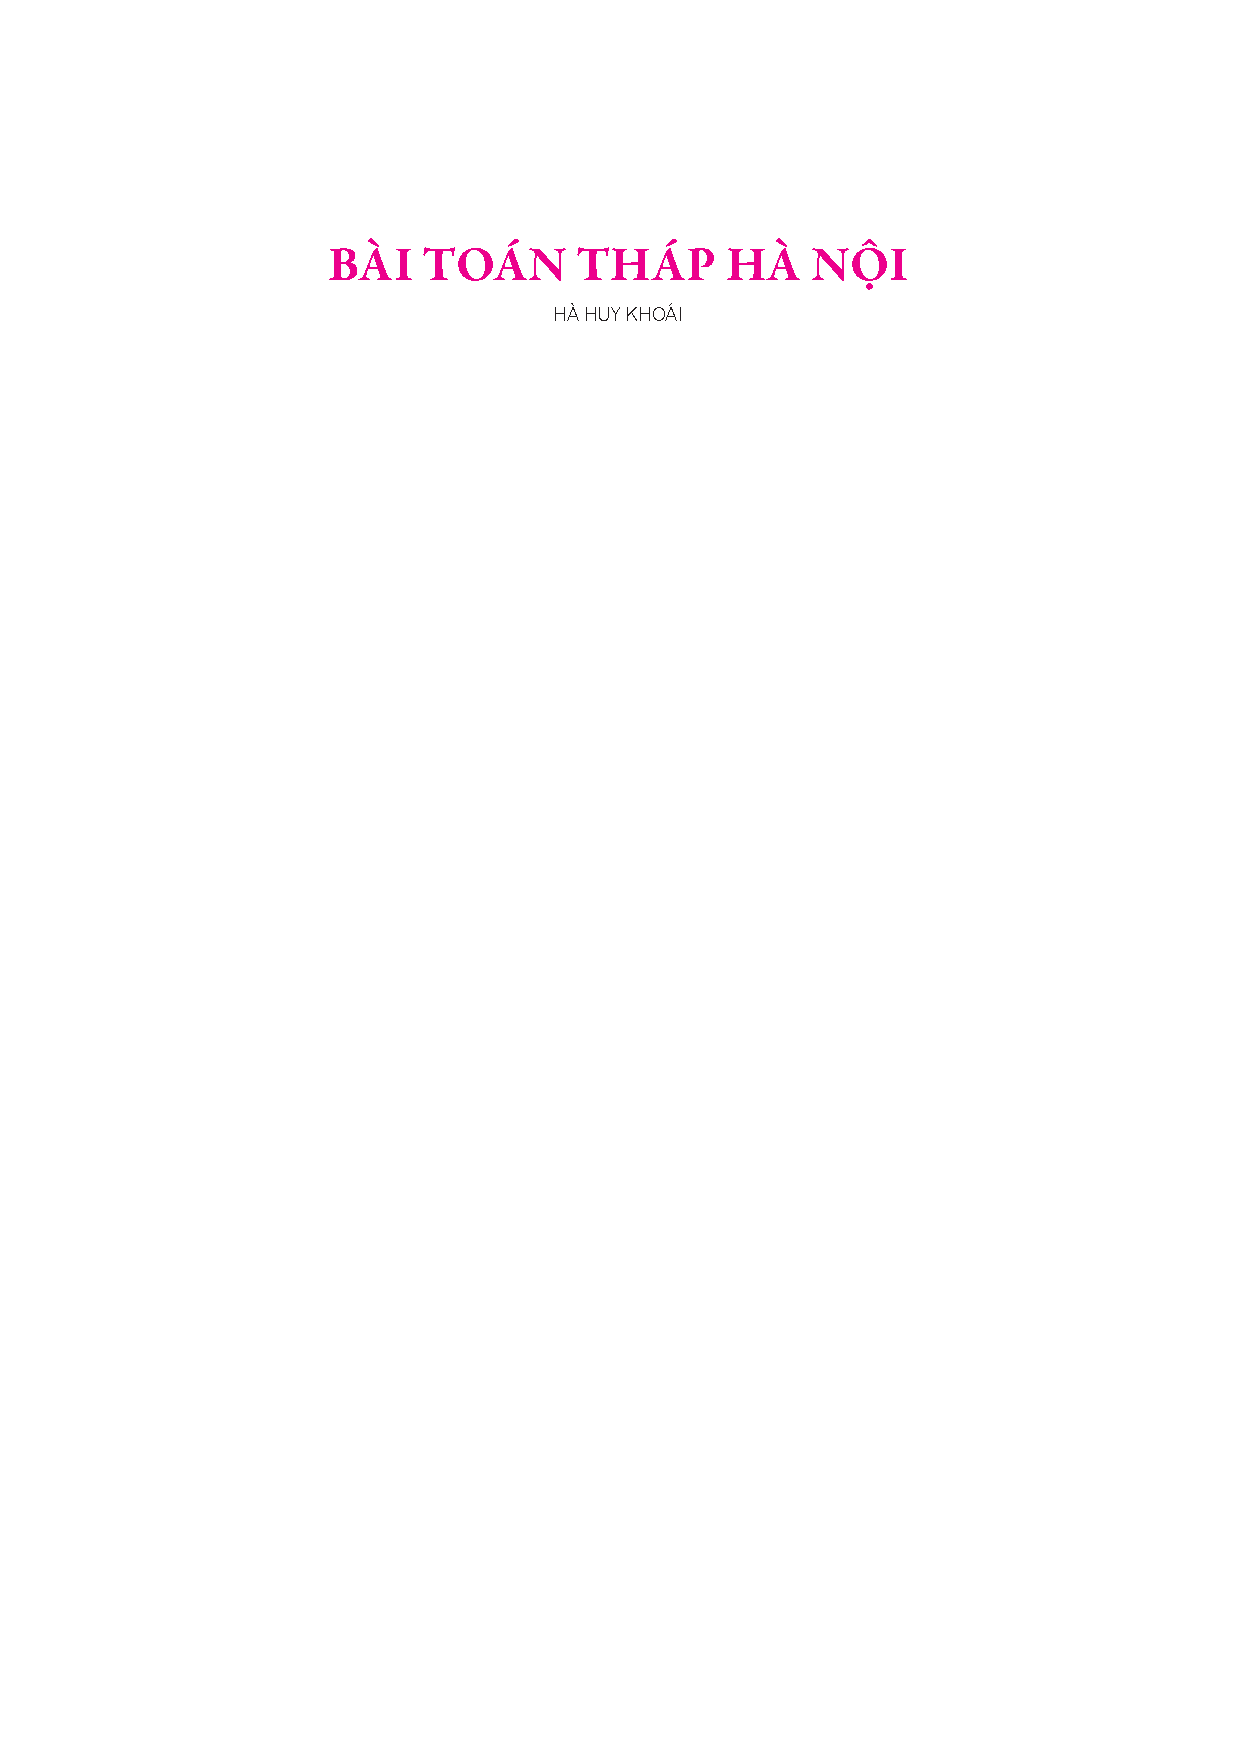
\includegraphics[scale=0.85]{../timhieulichsu/tieude.pdf}}} 
\centering
\endgroup

\vspace*{35pt}

	Trò chơi “Tháp Hà Nội”, xếp những miếng gỗ trên ba chiếc cọc, đã rất quen thuộc với các bạn nhỏ Việt Nam cũng như nhiều bạn nhỏ trên thế giới. Thật là tuyệt vời khi một trò chơi nổi tiếng trên thế giới lại có tên liên quan đến Thủ đô của nước ta đúng không. Các bạn đã biết về xuất xứ cùng với nhiều điều thú vị xung quanh bài toán “Tháp Hà Nội” chưa? Chúng ta hãy cùng ngược dòng thời gian để tìm hiểu qua bài viết dưới đây nhé.
	\vskip 0.1cm
	Năm $1883$, Eduard Lucas (Claus) công bố  bức tranh quảng cáo ``Tháp Hà Nội --  trò chơi thực sự nát óc xứ Annnam":
	\begin{figure}[H]
		\centering
		\vspace*{-5pt}
		\captionsetup{labelformat= empty, justification=centering}
		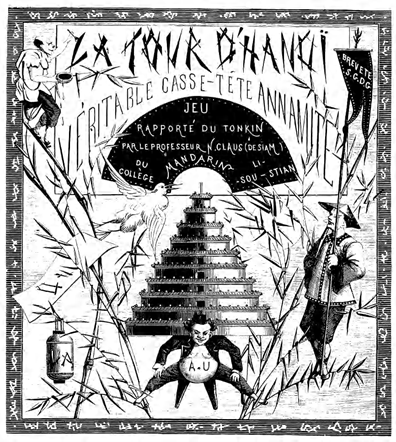
\includegraphics[width=0.4\linewidth]{1.1}
	%	\caption{\textit{\color{toancuabi}Hình $1$.}}
		\vspace*{-10pt}
	\end{figure}
	Một năm sau, Lucas viết bài ``Tháp Hà Nội , trò chơi toán học" đăng ở Tạp chí Science et Nature, số $1$ ($1884$) tr. $127-128$. Có thể xem đó ngày khai sinh của ``Bài toán Tháp Hà Nội", một trong những bài toán nổi tiếng của toán học. Cho đến ngày nay, vẫn còn rất nhiều công trình nghiên cứu về bài toán ``Tháp Hà Nội" và những mở rộng của nó, vẫn còn nhiều giả thuyết đang chờ câu trả lời.
	\vskip 0.1cm
	Hình sau đây là bức ảnh chụp từ hiện vật trưng bày trong ``Musée des arts et métiers--Cnam Paris" (Bảo tàng nghệ thuật và thủ công Paris). 
		\begin{wrapfigure}{l}{0.4\textwidth}
		\centering
%		\vspace*{-5pt}
		\captionsetup{labelformat= empty, justification=centering}
		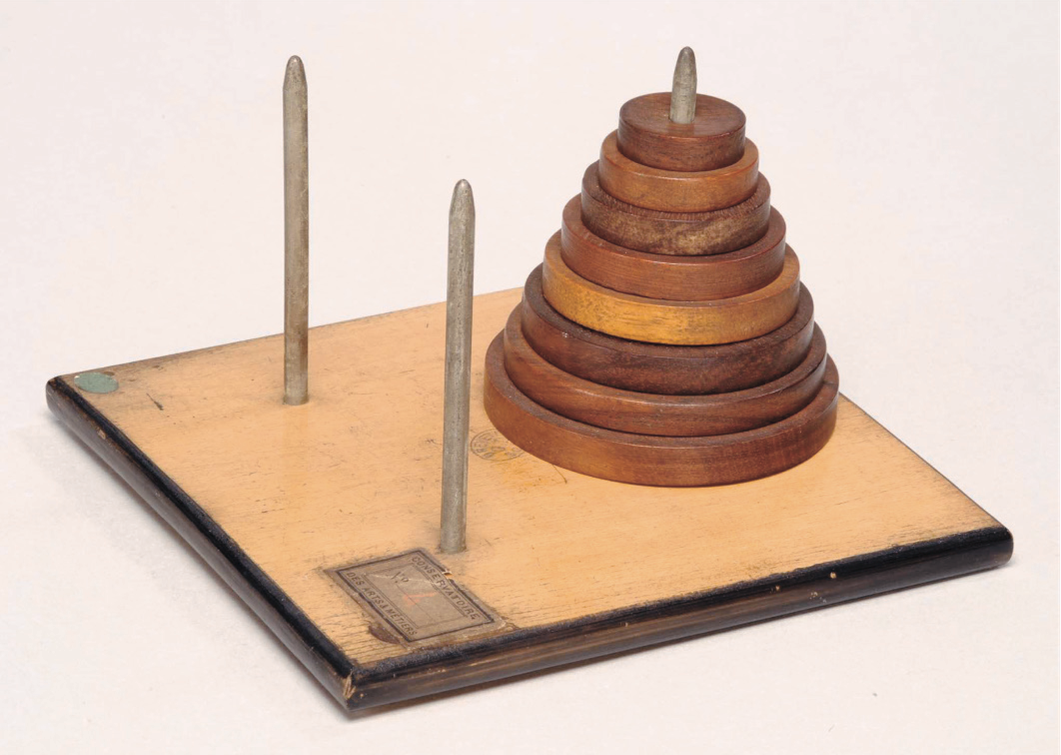
\includegraphics[width=1\linewidth]{2.1}
		%	\caption{\textit{\color{toancuabi}Hình $1$.}}
		\vspace*{-15pt}
	\end{wrapfigure}
	Ta có ba cái cọc, và  $8$ cái đĩa với kích thước khác nhau đôi một. Bài toán đặt ra là di chuyển toàn bộ $8$ cái đĩa sang một cọc khác, sao cho vẫn giữ được thứ tự các đĩa với bán kính lớn dần từ trên xuống dưới. Quy tắc di chuyển: mỗi lần chỉ được chuyển một đĩa, và không bao giờ được đặt một đĩa lên đĩa khác có bán kính nhỏ hơn. Điều này có thể làm được nhờ sử dụng cọc ``trung gian".
	\vskip 0.1cm
	Các bạn thử hình dung xem ta sẽ cần làm bao nhiêu phép chuyển đĩa?
	\vskip 0.1cm
	Trước hết, ta thử làm bài toán dễ hơn: trên cọc chỉ có $2$ đĩa. Rõ ràng chỉ cần chuyển đĩa nhỏ sang cọc trung gian, đĩa lớn sang cọc còn lại, rồi chuyển đĩa nhỏ lên cọc đó. Số bước chuyển là $3$.
	\vskip 0.1cm
	Nếu có $3$ đĩa trên cọc thì sao? Giả sử các đĩa đang ở cọc $A$, và ta cần chuyển sang cọc $C$. Ta chuyển hai đĩa trên cùng sang cọc  trung gian $B$, rồi chuyển đĩa to nhất sang cọc $C$. Sau đó chỉ cần chuyển hai đĩa từ cọc $B$ sang cọc $C$. Phương pháp chuyển $2$ đĩa từ cọc này sang cọc khác thì ta đã biết. Như vậy, số phép chuyển phải làm khi có $3$ đĩa bằng $2$ lần số phép chuyên khi có $2$ đĩa, cộng thêm $1$ phép chuyển (đĩa to nhất). 
	\vskip 0.1cm
	Như vậy, số bước chuyển cần thiết của $3$ đĩa là: $2\times 3 + 1 = 7$. Bằng quy nạp, dễ chứng minh nếu $N$ là số phép chuyển khi có $n$ đĩa thì với $(n+1)$ đĩa, ta có thể thực hiện nhiệm vụ với $(2N+1)$ phép chuyển. Từ đó, dễ suy ra, nhiệm vụ đặt ra trong bài toán ``Tháp Hà Nội" với $n$ đĩa có thể thực hiện với $2^n- 1$  phép chuyển.
	\vskip 0.1cm
	Có thể chứng minh $2^n - 1$  là số phép dịch chuyển tối thiểu cần thiết, nghĩa là không có cách gì thực hiện nhiệm vụ với số phép dịch chuyển ít hơn.
	\vskip 0.1cm
	Người ta cho rằng, bài toán ``Tháp Hà Nội" lấy ý tưởng từ câu chuyện cổ Ấn Độ sau đây.
	\vskip 0.1cm
	``Trong ngôi đền vĩ đại ở Benares, bên dưới mái vòm đánh dấu trung tâm thế giới, người ta đặt một chiếc đĩa bằng đồng, trên đó gắn cố định ba chiếc cọc kim cương, mỗi chiếc cao một mét và dày như thân của một con ong. Trên một trong những chiếc cọc  kim cương đó, vào buổi sáng tạo, Thượng Đế đặt $64$ chiếc đĩa bằng vàng nguyên chất, theo thứ tự to dần từ trên xuống dưới.  Ngày đêm không ngừng, những con quỷ chuyển các đĩa từ cọc kim cương này sang cọc kim cương khác theo nguyên tắc không được di chuyển nhiều hơn một đĩa cùng một lúc, và không được đặt đĩa nào lên trên cái nhỏ hơn nó. Khi $64$ chiếc  đĩa  được chuyển xong thì tiếng sét sẽ nổ ra, và thế giới tan biến".
	\vskip 0.1cm
	Những suy luận trên đây chỉ ra rằng, số phép dịch chuyển mà lũ quỷ phải làm ít nhất là
	\begin{align*}
		2^{64} - 1= 18{.}446{.}744{.}073{.}709{.}551{.}615.
	\end{align*}
	Giả sử lũ quỷ rất thạo ``thuật toán dịch chuyển", và mỗi giây chúng chuyển được một đĩa, thì phải mất khoảng $585$ tỷ năm. Có lẽ dù không có lũ quỷ, trái đất của chúng ta cũng không tồn tại được lâu đến thế!
	\vskip 0.1cm
	Từ sau khi ra đời, bài toán ``Tháp Hà Nội" nhận được sự quan tâm lớn của các nhà toán học và những người làm \!... đồ chơi. Rất nhiều phiên bản của bài toán ``Tháp Hà Nội" xuất hiện, chẳng hạn như số cọc lớn hơn $3$, hoặc cách chơi có thay đổi. Cho đến ngày nay, ``Tháp Hà Nội" và những biến thể của nó vẫn là bài toán quan trọng trong toán học rời rạc, lý thuyết đồ thị, khoa học máy tính, và tô pô (chẳng hạn, bài toán về đường cong tự cắt tại mọi điểm của nó!). Thậm chí, ``Tháp Hà Nội" còn có ứng dụng rộng rãi trong nghiên cứu tâm lý học!
	\vskip 0.1cm
	Người ta cho rằng, sở dĩ bài toán ``Tháp Hà Nội" lôi cuốn được nhiều thế hệ các nhà toán học vì nó chứa đựng những yếu tố làm nên sức hấp dẫn của Toán học: đẹp, thú vị, hữu ích, và bất ngờ.
	\newpage
	\begingroup
	\AddToShipoutPicture*{\put(76,588){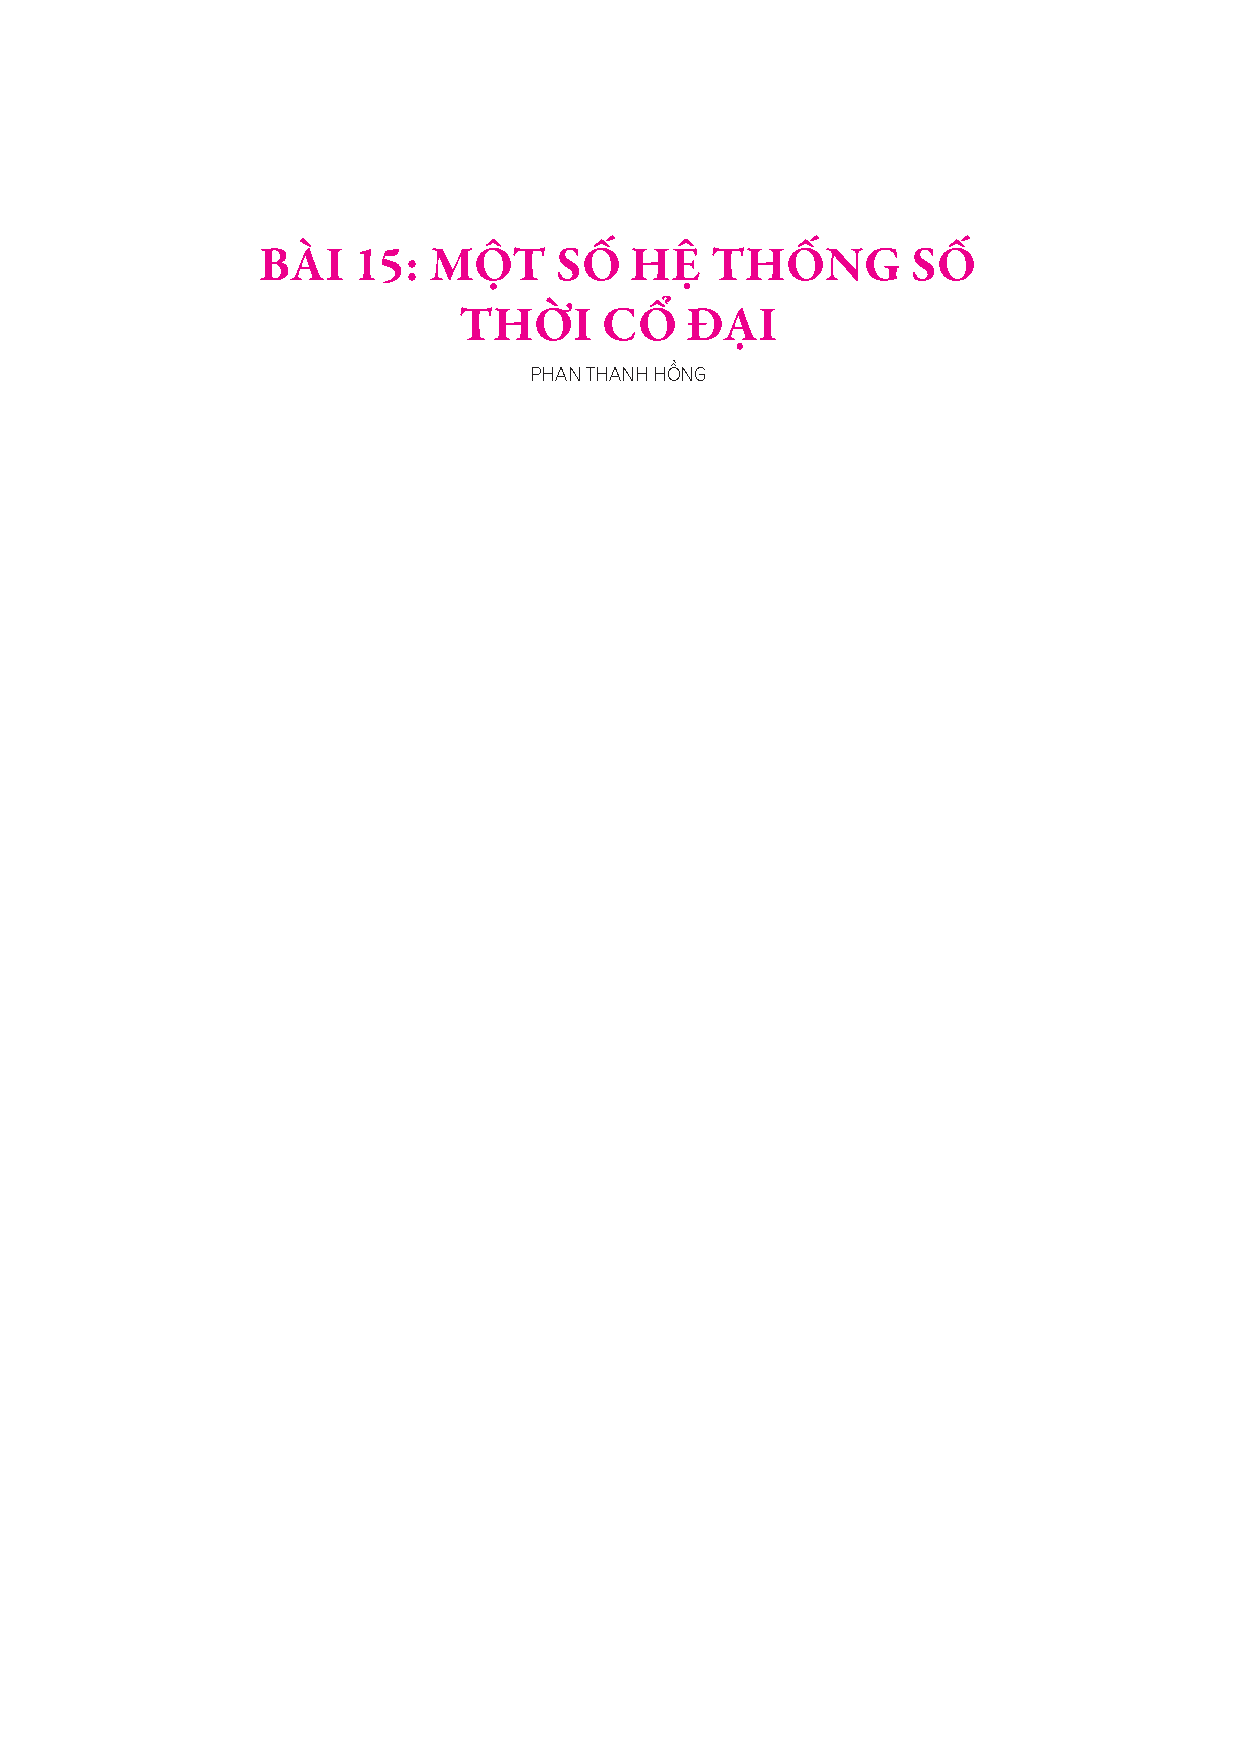
\includegraphics[scale=0.85]{../timhieulichsu/tieude2.pdf}}} 
	\centering
	\endgroup
	
	\vspace*{50pt}
	Mặc dù ngày nay, một số bộ lạc thổ dân sống ở rừng rậm Amazon, chỉ có những từ: ``một", ``hai" và ``nhiều" để nói về số lượng hay một số bộ khác khác chỉ đếm từ $1$ đến $5$; từ xa xưa người tiền sử đã đếm những số lớn hơn bằng cách đánh dấu lên đá hay xương động vật.
	\vskip 0.1cm
	\begin{wrapfigure}{r}{0.5\textwidth}
		\centering
		\vspace*{-5pt}
		\captionsetup{labelformat= empty, justification=centering}
		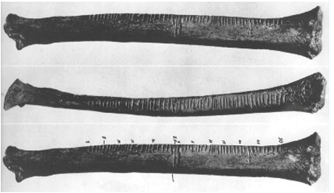
\includegraphics[width=1\linewidth]{1}
		\caption{\textit{\color{toancuabi}Hình $1$: Những mảnh xương chó sói trên có khía, được cho là ra đời cách đây $30{.}000$ năm và là công cụ để đếm của người thời tiền sử.}}
		\vspace*{-25pt}
	\end{wrapfigure}
	Từ hàng nghìn năm trước, ở những nền văn minh khác nhau, con người đã phát minh ra những hệ thống số để phục vụ mục đích đầu tiên là ghi nhớ những đại lượng lớn hơn. Những con số đó chính là khởi nguồn của toán học. Trong bài viết này chúng mình hãy cùng tìm hiểu về những con số của những nền văn minh khác nhau thời cổ đại nhé.
		\begin{figure}[H]
		\centering
%		\vspace*{-5pt}
		\captionsetup{labelformat= empty, justification=centering}
		\begin{tikzpicture}[scale=0.62]
			\draw [ fill=toanhocdoisong] (0,0) rectangle (5,1) node[pos=.5] {\tiny TIỀN SỬ};
			\draw [fill=duongvaotoanhoc] (5,0) rectangle + (4,1) node[pos=.5] {\tiny CỔ ĐẠI};
			\draw [fill=doisongtoanhoc] (9,0) rectangle + (3,1) node[pos=.5] {\tiny TRUNG ĐẠI};
			\draw [fill=timhieukhoahoc] (12,0) rectangle + (3,1) node[pos=.5] {\tiny CẬN ĐẠI};
			\draw [fill=diendantoanhoc] (15,0) rectangle + (3,1) node[pos=.5] {\tiny HIỆN ĐẠI};
			\draw[<->, line width=1.0mm, toancuabi] (0,-0.8) -- (18,-0.8);
			\draw[line width=1.0mm, timhieukhoahoc] (1,-1.1) -- (1,-0.5) node[mystyle] {$2.000.000$ năm trước};
			\draw[line width=1.0mm, timhieukhoahoc] (5,-1.1) -- (5,-0.5) node[mystyle] {$5.000$ năm trước};
			\draw[line width=1.0mm, timhieukhoahoc] (9,-1.1) -- (9,-0.5)  node[mystyle] { năm $500$};
			\draw[line width=1.0mm, timhieukhoahoc] (12,-1.1) -- (12,-0.5) node[mystyle] {năm $1.500$};
			\draw[line width=1.0mm, timhieukhoahoc] (15,-1.1) -- (15,-0.5) node[mystyle] {năm $1.800$};
			\draw[line width=1.0mm, timhieukhoahoc] (17.2,-1.1) -- (17.2,-0.5) node[mystyle] {năm $2022$} ;
			
		\end{tikzpicture}
		\vspace*{-10pt}
	\end{figure}
	Trước tiên, các em hãy quan sát những hình ảnh trong hình bên.  Em có đoán được chúng nói lên điều gì không? Chúng cùng nói về  một thứ. Đó là số $23$. Từ trên xuống, số $23$ lần lượt được viết trong hệ thống số của người Ai Cập, người Babylon, người Maya và người Trung Quốc thời cổ đại. 
	\vskip 0.1cm
		\begin{wrapfigure}{r}{0.35\textwidth}
		\centering
		\vspace*{-10pt}
		\captionsetup{labelformat= empty, justification=centering}
		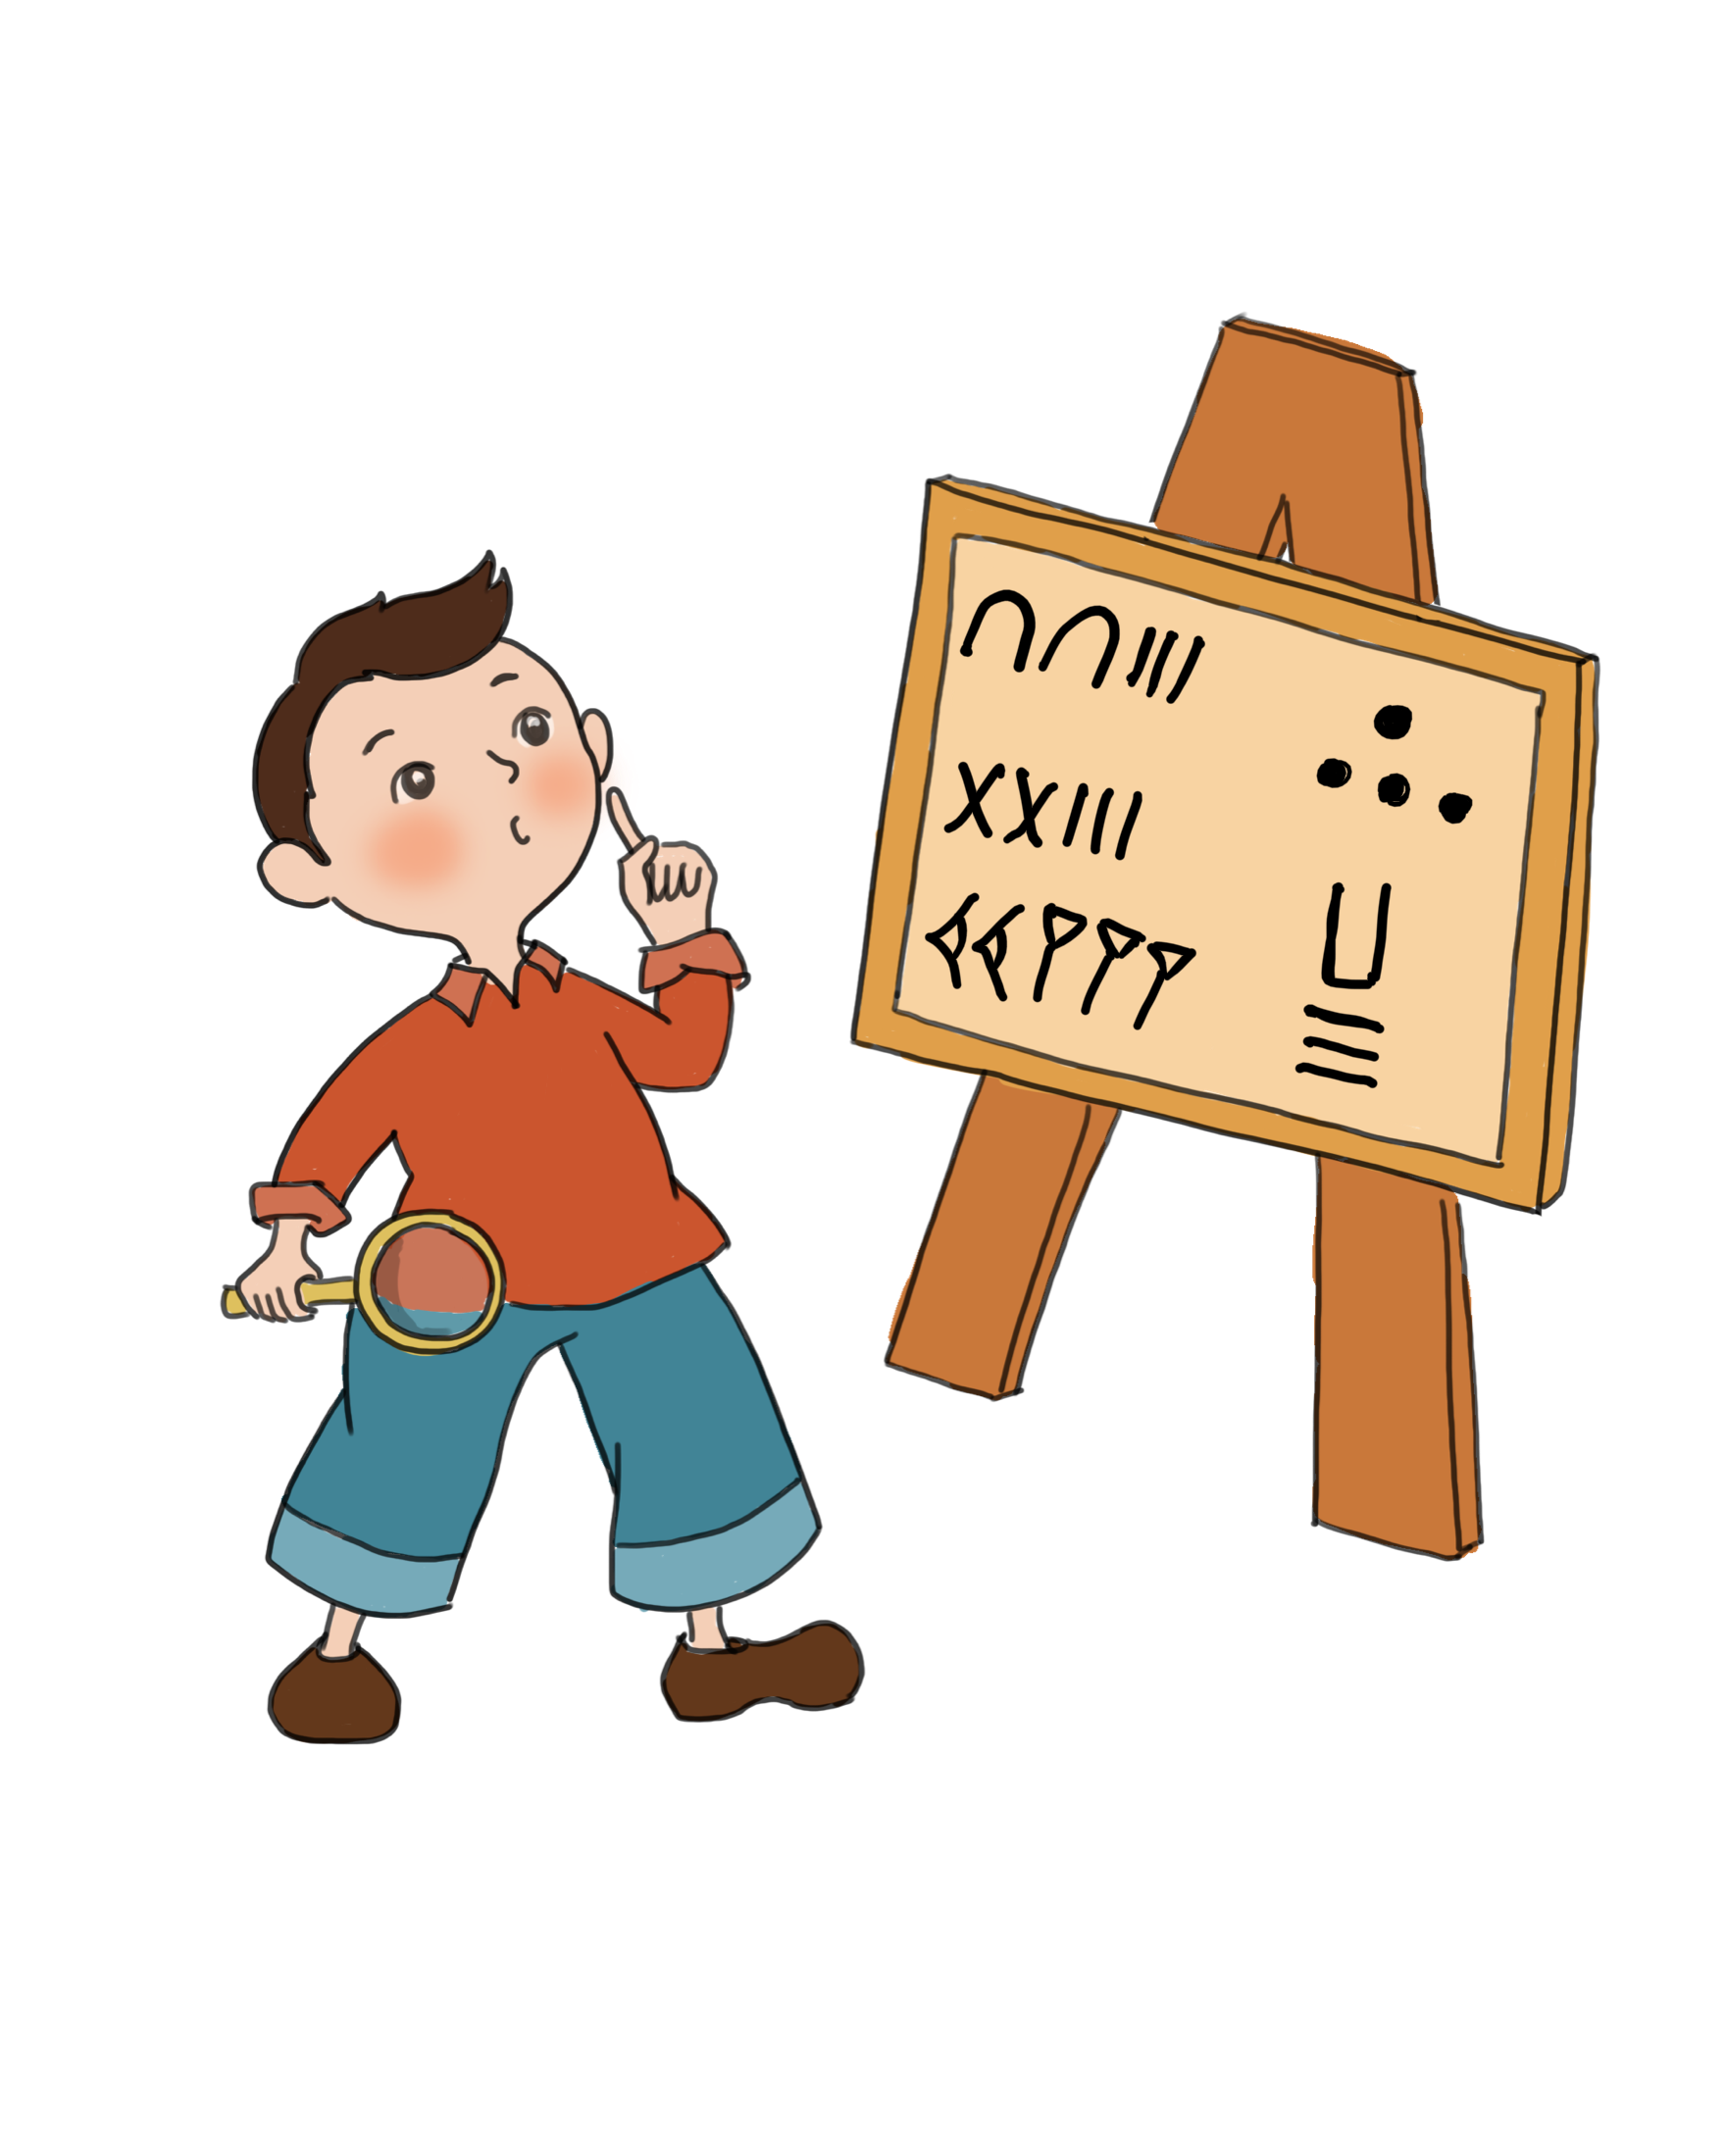
\includegraphics[width=1\linewidth]{20.12-pi}
		\vspace*{-30pt}
	\end{wrapfigure}
	Các em thấy chúng có điểm gì chung? Em có thể đoán xem kí hiệu nào biểu diễn hàng chục, hàng đơn vị không? Chúng khác cách chúng ta viết số $23$ ngày nay như thế nào?
	\vskip 0.1cm
	\textbf{\color{toancuabi}Số Ai Cập cổ}
	\vskip 0.1cm
	Ai Cập cổ đại, một trong những cái nôi văn minh của nhân loại, là vùng đất nằm dọc hai bên sông Nile, phía Bắc của châu Phi. Toán học đã xuất hiện ở đây cách đây hơn $5000$ năm. Những thành tựu toán học là một trong những yếu tố quan trọng giúp người Ai Cập cổ xây dựng nên những kim tự tháp mà một số vẫn còn tồn tại đến ngày nay. 
	\vskip 0.1cm
	Người Ai Cập cổ sử dụng những kí hiệu bằng hình ảnh để viết chữ và viết các số (được gọi là chữ viết \textit{tượng hình}). Những kí hiệu chữ số của họ như sau:
	\begin{table}[H]
		\vspace*{-5pt}
		\setlength{\tabcolsep}{4.1pt}
%			\renewcommand{\arraystretch}{1.1}
		\centering
		\resizebox{0.95\columnwidth}{!}{\begin{tabular}{|c|c|c|c|c|c|c|}
			\hline
			\multicolumn{7}{|c|}{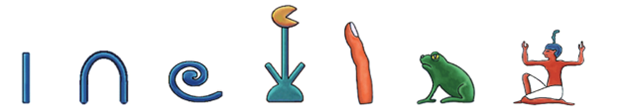
\includegraphics[width=0.95\linewidth]{2}}\\
			\hline
			$1$&$10$ &$100$&$1{.}000$&$10{.}000$&$100{.}000$&$1{.}000{.}000$\\
			\hline
			\shortstack{Gạch \\đứng}&\shortstack{Móng\\ ngựa}&\shortstack{Cuộn\\ dây}&\shortstack{Hoa \\sen}&\shortstack{Ngón\\ tay}&\shortstack{Con\\ ếch}&\shortstack{Vị \\thần}\\
			\hline
		\end{tabular}}
	\vspace*{-10pt}
	\end{table}
	Số $4$ được viết là 
\includegraphics{3} còn 
\includegraphics{4}  là số $7$. Để viết các số từ $10$ trở lên, người ta dùng thêm kí hiệu 
\includegraphics{5} (để biểu diễn số $10$), chẳng hạn số $17$ được viết là 
\includegraphics{5}
\includegraphics{4} và số $27$ được viết là  
\includegraphics{5}
\includegraphics{5}
\includegraphics{4}. Số lượng các kí hiệu 
\includegraphics{5} cho biết có bao nhiêu chục, số các kí hiệu $\mid$ cho biết có bao nhiêu đơn vị trong số được biểu diễn. Với những số từ $100$ trở đi họ dùng kí hiệu 
\includegraphics{6} (biểu diễn số $100$) và viết các số theo cách tương tự; và cứ như vậy cho những số lớn hơn. Để biết giá trị của số được biểu diễn ta cộng các giá trị ứng với những kí hiệu biểu diễn nó. Chẳng hạn, 
\includegraphics{6}
\includegraphics{6}
\includegraphics{5}
\includegraphics{5}
\includegraphics{5}
\includegraphics{3.1}   $=  100+ 100 + 10 + 10 + 10 + 1 + 1 + 1= 233$.
	\vskip 0.1cm
		\begin{wrapfigure}{l}{0.35\textwidth}
		\centering
		\vspace*{-5pt}
		\captionsetup{labelformat= empty, justification=centering}
		
\includegraphics[width=0.9\linewidth]{20.12-pi.1}
		\vspace*{-15pt}
	\end{wrapfigure}
	Ngày nay, ta dùng các hàng khác nhau để biểu diễn số: hàng đơn vị, hàng chục, hàng trăm,... Hàng chục đứng ngay trước hàng đơn vị và lớn gấp $10$ lần hàng đơn vị, hàng trăm đứng ngay trước hàng chục và lớn gấp $10$ lần hàng chục. Do đó, hệ thống số mà chúng ta sử dụng hiện nay trong đời sống là ``hệ cơ số $10$",  hay ``\textit{hệ thập phân}". Hệ thống số Ai Cập cổ cũng là một hệ cơ số $10$ nhưng việc viết các số phức tạp hơn so với cách viết ngày nay của chúng ta, nhất là với những số lớn. Chẳng hạn để viết số ${5.}412{.}316$ người Ai Cập cổ xưa cần dùng $22$ kí hiệu!
	\vskip 0.1cm
	$5412316    =$ 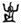
\includegraphics{7}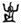
\includegraphics{7}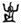
\includegraphics{7}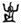
\includegraphics{7}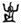
\includegraphics{7}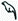
\includegraphics{8}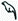
\includegraphics{8}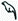
\includegraphics{8}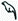
\includegraphics{8}
\includegraphics{9}
\includegraphics{10}
\includegraphics{10}
\includegraphics{11}
\includegraphics{11}
\includegraphics{11}
\includegraphics{5}
\includegraphics{12}
\includegraphics{12}
\includegraphics{12}
\includegraphics{12}
\includegraphics{12}
\includegraphics{12} 
	\vskip 0.1cm 
	
	\begin{wrapfigure}{r}{0.3\textwidth}
		\vspace*{-10pt}
		\centering
		\captionsetup{labelformat=empty, justification=centering}
		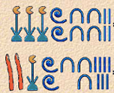
\includegraphics[scale=1]{13}
		\vspace*{-10pt}
	\end{wrapfigure}                          
	Em hãy viết các số Ai Cập trong hình sau đây theo cách thông thường nhé.    
	\vskip 0.1cm
	\textbf{\color{toancuabi}Số La Mã}
	\vskip 0.1cm
	Các em có nhìn thấy các kí hiệu I, II, ... X trên mặt đồng hồ, trong sách vở, trên bảng khi cô giáo đánh số các mục trong bài giảng? Đó là các số La Mã. La Mã là tên gọi một quốc gia cổ đại thuộc châu Âu mà có thời kì từng thống trị một vùng đất rộng lớn của châu lục này. Người La Mã sử dụng một số chữ cái từ bảng chữ cái của họ để biểu diễn những chữ số khác nhau.
	\begin{figure}[H]
		\centering
		\vspace*{-10pt}
		\captionsetup{labelformat= empty, justification=centering}
		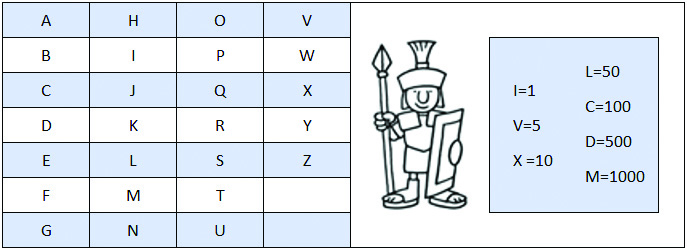
\includegraphics[width=1\linewidth]{14a}
		\caption{\small\textit{Chú thích: các chữ cái và chữ số La Mã}}
		\vspace*{-10pt}
	\end{figure}
	Số $4$ được viết là IV, còn số $6$ là VI. Khi một chữ số lớn được viết ngay trước  một chữ số nhỏ hơn hay bằng nó, ta cộng chúng lại với nhau để được con số cần biểu diễn, như trường hợp số $6=$ VI. Ngược lại, ta thực hiện phép trừ, giống như trường hợp số $4=$ IV.
	\begin{table}[H]
		\vspace*{-5pt}
		\centering
			\begin{tabular}{|l l|l l|}
			\hline
			IV $=4$:&    V$-$I $=$ IV & VI $=6$:&    V$+$I =VI\\
			&$5-1=4$ & &$5+1=6$\\
			\hline
		\end{tabular}
		\vspace*{-10pt}
	\end{table}
	Tương tự, ta có
	\begin{table}[H]
		\vspace*{-5pt}
		\centering
		\resizebox{1\textwidth}{!}{\begin{tabular}{|l l|l l|}
			\hline
			XXXII $= 32$:&    X$+$X$+$X$+$I$+$I $=$ XXXII& XL$= 40$:&     L $-$ X = XL\\
			&$10 +10 +10+1+1=32$&	&$50 - 10 = 40$\\
			\hline
		\end{tabular}}
		\vspace*{-10pt}
	\end{table}
	Theo cách người La Mã viết số, một chữ số nhỏ đứng trước chữ số số lớn hơn, ta trừ số lớn cho số bé. Trong đó I, V chỉ được trừ từ những giá trị không quá X. Ví dụ, ta có thể viết IX nhưng không thể viết IL; X, L chỉ được trừ bởi những chứ số không vượt quá C; C, D chỉ được trừ cho những chữ số không vượt quá M. Ngoài ra, còn có những quy tắc khác như sau:
	\vskip 0.1cm
	-- Luôn viết số bằng cách dùng ít kí hiệu nhất, chẳng hạn ta viết XX để biểu diễn $20$ thay vì VVVV.
	\vskip 0.1cm
	-- Không có nhiều hơn $3$ kí tự giống nhau trong một hàng (đơn vị, chục, trăm,..). Ví dụ ta viết XIV thay vì XIIII để biểu diễn $14$.
	\vskip 0.1cm
	-- Để biểu diễn số gấp hơn $1000$ lần, người La Mã dùng vạch ngang phía trên các dãy chữ số, ví dụ $\overline{VI}II=6\times 1000+2=6002$. Ở đây, VI có thêm vạch ngang trên đầu biểu diễn giá trị $6\times 1000 = 6000$. Những chữ số có vạch ngang trên đầu đứng trước các chữ số còn lại.
	\vskip 0.1cm
	Không đặt nhiều hơn $1$ số nhỏ đứng trước $1$ số lớn. Ví dụ ta không viết IIX để biểu diễn $8$.
	\vskip 0.1cm
	Để dễ dàng viết số La Mã, ta viết theo từng hàng từ  lớn đến nhỏ (như các số mà ngày nay chúng ta dung). Ví dụ, để viết số $645$, ta viết $600$ trước (DC), rồi $40$ (XL) và cuối cùng là $5$ (V). Vậy $DCXLV=645$.
	\vskip 0.1cm
	\textbf{\color{toancuabi}Số Babylon}
	\vskip 0.1cm
	\begin{wrapfigure}{r}{0.4\textwidth}
		\centering
		\vspace*{-15pt}
		\captionsetup{labelformat= empty, justification=centering}
		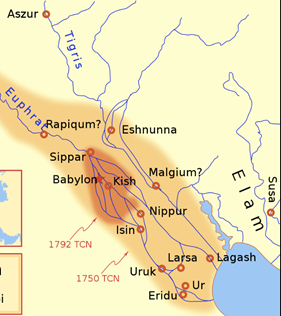
\includegraphics[width=1\linewidth]{17.1}
		%	\caption{\textit{\color{toancuabi}Hình $1$.}}
		\vspace*{-30pt}
	\end{wrapfigure}
	Người Babylon, sống vào khoảng $5000$ năm trước ở vùng đất Lưỡng Hà (một khu vực ở phía Tây của  Châu Á), nổi tiếng vì khả năng toán học của họ. Họ đã tạo ra những công cụ tính toán thiên văn, hình học đáng kinh ngạc và họ đã phát minh ra bàn tính.
	\vskip 0.1cm
	Trong hệ thống số của mình, ban đầu người Babylon chỉ sử dụng $2$ kí hiệu 
	\begin{table}[H]
		\vspace*{-5pt}
		\centering
		\begin{tabular}{|c|c|}
			\hline
			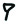
\includegraphics[scale=0.7]{15}&$1$\\
			\hline
			\includegraphics[scale=0.65]{16}&$10$\\
			\hline
		\end{tabular}
		\vspace*{-5pt}
	\end{table}
	để viết số từ $1$ tới $60$, chẳng hạn số $7$ là  \includegraphics[scale=0.75]{17}, số $27$ là  \includegraphics[scale=0.75]{16}\includegraphics[scale=0.75]{16}\includegraphics[scale=0.75]{17}. 	 
	\vskip 0.1cm
	Những kí hiệu này được sử dụng tương tự như những chữ số La Mã (bằng cách cộng các kí hiệu xuất hiện trong số được biểu diễn). Số \includegraphics[scale=0.75]{18} được viết bởi $2$ kí hiệu \includegraphics[scale=0.75]{16} để biểu diễn $2$ chục, và $7$ kí hiệu \includegraphics[scale=0.75]{15}  cho $7$ đơn vị. Do vậy \includegraphics[scale=0.75]{18}  $=27$.
	\vskip 0.1cm
	Sau đó, một kí hiệu mới được sử dụng để biểu diễn chữ số $0$ (các em có thấy nó là chữ số $1$ viết ngiêng?)
	\includegraphics[scale=0.75]{15.1}
	\vskip 0.1cm
	Để viết những số từ $60$ trở đi, người Babylon xếp các kí hiệu theo các nhóm. Điều này giống như ngày nay các em viết $159$ bằng cách viết số $1$ đầu tiên ứng với hàng trăm, số $5$ tiếp theo ở hàng chục và cuối cùng là số $9$ ở hàng đơn vị. Như vậy $159 = 1 \times 100+ 5 \times 10+ 9$.
	\vskip 0.1cm
	Để viết số $63$, người Babylon viết kí hiệu  \includegraphics[scale=0.85]{15}  ở hàng $60$ và ba kí hiệu \includegraphics[scale=0.85]{15}  ở hàng đơn vị và để khoảng trống để phân biệt hai nhóm (tức hai hàng: hàng $60$ và hàng đơn vị) \includegraphics[scale=0.85]{15}\includegraphics[scale=0.85]{15}\includegraphics[scale=0.85]{15}
	\vskip 0.1cm
	\begin{wrapfigure}{l}{0.4\textwidth}
		\centering
		\vspace*{-15pt}
		\captionsetup{labelformat= empty, justification=centering}
		\includegraphics[width=1\linewidth]{20.12-pi.2}
		\vspace*{-25pt}
	\end{wrapfigure}
	\vskip 0.1cm
	Vậy \includegraphics[scale=0.85]{16.1}. Trong cách viết này, ta thấy có $4$ kí hiệu \includegraphics[scale=0.85]{15}   nhưng kí hiệu đầu tiên được viết tách biệt so với $3$ cái còn lại để biểu diễn số $1$ lần $60$ tức $60$, $3$ kí hiệu còn lại biểu diễn số $3$ và như vậy ta có số $60+3 =63$.
	\vskip 0.1cm
	Điều này giống như chúng ta viết chữ số $1$ ở hàng chục và chữ số $1$ ở hàng đơn vị để biểu diễn số $11$: nó có nghĩa là $1$ chục và $1$ đơn vị. Trong  hệ thống số  Babylon cổ, nó có nghĩa là $1$ lần $60$  và $1$.
	\vskip 0.1cm
	Để hiểu rõ hơn, ta hãy viết số chín mươi ba theo hệ số hiện đại. Việc này thật dễ dàng phải không? Tuy nhiên để hiểu cách viết của người Babylon ta sẽ thực hiện theo cách như sau: do các số của chúng ta ngày nay sử dụng hệ cơ số $10$, ta chia chín mươi ba cho $10$ được thương là $9$, nên ta viết $9$ vào hàng chục
	\begin{figure}[H]
		\centering
		\vspace*{-5pt}
		\captionsetup{labelformat= empty, justification=centering}
		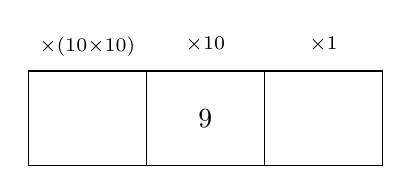
\begin{tikzpicture}[xscale=1.5,yscale=1.2]
			\draw (0,0) grid (3,1);
			\draw (1.5,0.5) node {$9$};
			\draw (0.5,1.05) node[above] {$\scriptstyle\times(10\times10)$};
			\draw (1.5,1.1) node[above] {$\scriptstyle\times10$};
			\draw (2.5,1.1) node[above] {$\scriptstyle\times1$};
		\end{tikzpicture}
		\vspace*{-10pt}
	\end{figure}
	Phép chia đó có số dư $3$ nên ta viết $3$ vào hàng đơn vị
	\begin{figure}[H]
		\centering
		\vspace*{-5pt}
		\captionsetup{labelformat= empty, justification=centering}
		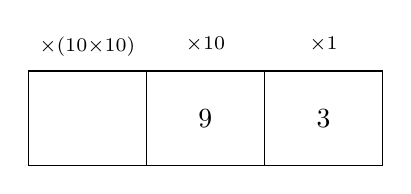
\begin{tikzpicture}[xscale=1.5,yscale=1.2]
			\draw (0,0) grid (3,1);
			\draw (1.5,0.5) node {$9$};
			\draw (2.5,0.5) node {$3$};
			\draw (0.5,1.05) node[above] {$\scriptstyle\times(10\times10)$};
			\draw (1.5,1.1) node[above] {$\scriptstyle\times10$};
			\draw (2.5,1.1) node[above] {$\scriptstyle\times1$};
		\end{tikzpicture}
		\vspace*{-10pt}
	\end{figure}
	Vậy là ta viết: $93$.
	\vskip 0.1cm
	Thế còn người Babylon viết số $93$ trong hệ thống số của họ như thế nào?
	\vskip 0.1cm
	\textit{Hệ thống số Babylon sử dụng hệ cơ số $60$:} ta chia $93$ cho $60$ được thương là $1$ nên ta viết $1$ ở hàng $60$
	\begin{figure}[H]
		\centering
		\vspace*{-5pt}
		\captionsetup{labelformat= empty, justification=centering}
		\begin{tikzpicture}[xscale=1.5,yscale=1.2]
			\draw (0,0) grid (3,1);
			\node[inner sep=0pt] (mouse) at (1.5,0.5){\includegraphics[scale=1]{27a}};
			\draw (0.5,1.05) node[above] {$\scriptstyle\times(60\times60)$};
			\draw (1.5,1.1) node[above] {$\scriptstyle\times60$};
			\draw (2.5,1.1) node[above] {$\scriptstyle\times1$};
		\end{tikzpicture}
		\vspace*{-10pt}
	\end{figure}
	Phép chia có số dư là $33$, nên ta sẽ viết $33$ ở hàng đơn vị. Số $33$ được biểu diễn bởi $3$ kí tự mười cộng với $3$. Nên ta đặt $3$ kí tự $10$ và $3$ kí tự $1$ vào hàng đơn vị như sau
	\begin{figure}[H]
		\centering
		\vspace*{-5pt}
		\captionsetup{labelformat= empty, justification=centering}
		\begin{tikzpicture}[xscale=1.5,yscale=1.2]
			\draw (0,0) grid (3,1);
			\node[inner sep=0pt] (mouse) at (1.5,0.5){\includegraphics[scale=1]{27a}};
			\node[inner sep=0pt] (mouse) at (2.5,0.5){\includegraphics[scale=1]{22a}};
			\draw (0.5,1.05) node[above] {$\scriptstyle\times(60\times60)$};
			\draw (1.5,1.1) node[above] {$\scriptstyle\times60$};
			\draw (2.5,1.1) node[above] {$\scriptstyle\times1$};
		\end{tikzpicture}
		\vspace*{-10pt}
	\end{figure}
	Vậy \includegraphics{23}  $= 93$.
	\vskip 0.1cm
	Tiếp theo, chúng ta hãy thử viết số lớn hơn. Chúng ta hãy cùng viết số $3604$ bằng các chữ số Babylon nhé. Số $3604$ lớn hơn $60\times 60=3600$, nên ta cần biểu diễn số này từ hàng thứ $3$ tính từ hàng đơn vị. Ta chia số $3604$ cho $3600$ được thương là $1$ nên ta viết kí tự số \includegraphics{15}  vào hàng $60\times60$
	\begin{figure}[H]
		\centering
		\vspace*{-5pt}
		\captionsetup{labelformat= empty, justification=centering}
		\begin{tikzpicture}[xscale=1.5,yscale=1.2]
			\draw (0,0) grid (3,1);
			\node[inner sep=0pt] (mouse) at (0.5,0.5){\includegraphics[scale=1]{27a}};
			\draw (0.5,1.05) node[above] {$\scriptstyle\times(60\times60)$};
			\draw (1.5,1.1) node[above] {$\scriptstyle\times60$};
			\draw (2.5,1.1) node[above] {$\scriptstyle\times1$};
		\end{tikzpicture}
		\vspace*{-10pt}
	\end{figure}
	Số dư của phép chia là $4$ nhỏ hơn $60$ nên ta viết kí hiệu số $0$ ( \includegraphics{15.1}) vào hàng $60$, và $4$ (\includegraphics{15}\includegraphics{15}\includegraphics{15}\includegraphics{15}    ) vào hàng đơn vị. 
	\begin{figure}[H]
		\centering
		\vspace*{-5pt}
		\captionsetup{labelformat= empty, justification=centering}
		\begin{tikzpicture}[xscale=1.5,yscale=1.2]
			\draw (0,0) grid (3,1);
			\node[inner sep=0pt] (mouse) at (0.5,0.5){\includegraphics[scale=1]{27a}};
			\node[inner sep=0pt] (mouse) at (1.5,0.5){\includegraphics[scale=1]{27b}};
			\node[inner sep=0pt] (mouse) at (2.5,0.5){\includegraphics[scale=1]{27c}};
			\draw (0.5,1.05) node[above] {$\scriptstyle\times(60\times60)$};
			\draw (1.5,1.1) node[above] {$\scriptstyle\times60$};
			\draw (2.5,1.1) node[above] {$\scriptstyle\times1$};
		\end{tikzpicture}
		\vspace*{-10pt}
	\end{figure}
	Vậy, số $3604$ được người Babylon viết như sau:
	\begin{figure}[H]
		\centering
		\vspace*{-5pt}
		\captionsetup{labelformat= empty, justification=centering}
		\includegraphics[width=0.4\linewidth]{27}
		%	\caption{\textit{\color{toancuabi}Hình $1$.}}
		\vspace*{-10pt}
	\end{figure}
	\textit{Số của người Ai Cập, La Mã hay chúng ta ngày nay được gọi là hệ sơ số $10$ còn số của người Babylon là cơ số $60$. Do số $60$ chia hết cho nhiều số: $1,2,3,4,5,6, 10, 12, 15, 20,30$ và $60$ việc chia các đại lượng được thực hiện dễ dàng hơn, ít phải dùng đến các phân số. Việc sử dụng đơn vị thời gian: $1$ phút $= 60$ giây, $1$ giờ $= 60$ phút ngày nay là một ảnh hưởng của người Babylon đấy.}
	\vskip 0.1cm
	\textbf{\color{toancuabi}Số Maya}
	\vskip 0.1cm
	\begin{wrapfigure}{r}{0.47\textwidth}
		\centering
		\vspace*{-15pt}
		\captionsetup{labelformat= empty, justification=centering}
		\includegraphics[width=1\linewidth]{28}
		\caption{\textit{Kim tự tháp Tikal\\ của người Maya}}
		\vspace*{-20pt}
	\end{wrapfigure}
	Người Maya  được cho là đã xuất hiện từ rất xa xưa. Họ đã xây dựng hệ thống lịch chính xác và toán học của họ là đại diện tiêu biểu cho toán học của các cộng đồng dân cư ở châu Mỹ thời cổ đại.
	
	Nói về hệ thống số,  người Maya  cổ dùng hệ cơ số $20$, gồm $3$ kí hiệu:  (\includegraphics{29}),  \includegraphics{30}, \includegraphics{31}  ứng với $0,1, 5$ và biểu diễn số theo chiều dọc. Chữ số ở hàng cao hơn được viết phía trên, chữ số ở hàng thấp hơn được viết phía dưới. Điều này tương tự chúng ta viết số ngày nay: ta đặt số ở hàng cao hơn bên trái còn số ở hàng thấp hơn bên phải. 
	\begin{table}[H]
		\vspace*{-5pt}
		\centering
		\setlength{\tabcolsep}{4.5pt}
		\renewcommand{\arraystretch}{1.3}
		\begin{tabular}{|l|l|}
			\hline
			$10^3 = 10\!\times\! 10 \!\times\! 10 =1000$& hàng nghìn\\
			\hline
			$10^2 = 10\!\times\! 10 =100$& hàng trăm\\
			\hline
			$10^1 = 10$& hàng chục\\
			\hline
			$10^0 = 1$& hàng đơn vị\\
			\hline
		\end{tabular}
		%		\vspace*{-5pt}
	\end{table}
	Do sử dụng hệ cơ số $20$,  số Maya được biểu diễn trong phần bên phải của bảng  sau chính là số  $1\times 8000+ 0\times 400+ 10\times20+ 7\times1= 8207$. Bởi vì, ta  thấy  \includegraphics[scale=0.5]{33},  \includegraphics[scale=0.5]{34},  \includegraphics[scale=0.5]{35}, \includegraphics[scale=0.5]{36}  ứng với $1, 0, 10, 7$  lần lượt ở các hàng $8000$, $400$, $20$ và đơn vị. Chú ý rằng, trong một hàng, số có giá trị cao hơn lại được viết phía dưới số có giá trị lớn hơn chẳng hạn  \includegraphics[scale=0.5]{36}:  hai kí tự \includegraphics{37} (số $1$) được viết bên trên kí tự \includegraphics{38} (số $5$). Kí hiệu \includegraphics{39} để biểu diễn $0$ ở một hàng giống như ta viết $101$ và giúp ta phân biệt số $101$ với số $11$. Điều này cũng tương tự như ở hệ thống số Babylon. 
	\vskip 0.1cm
	\begin{wrapfigure}{l}{0.4\linewidth}
		\centering
		\vspace*{-20pt}
		\captionsetup{labelformat= empty, justification=centering}
		\includegraphics[width=0.95\linewidth]{32}
		\vspace*{-20pt}
	\end{wrapfigure}
	\vskip 0.1cm
	Người ta cho rằng hệ cơ số $10$ được dùng phổ biến vì con người có $10$ ngón tay (các em nhỏ rất hay xòe tay để đếm phải không nào?),  còn người Maya vốn không đi giày nên họ đếm bằng cả các ngón chân nữa. Họ dùng hệ cơ số $20$ là vì thế!
	\vskip 0.1cm
	\textbf{\color{toancuabi}Số Trung Hoa cổ}
	\vskip 0.1cm
	Trung Hoa cổ đại là một trong những nền văn minh cổ lớn của thế giới. Người Trung Hoa dưới thời nhà Thương (khoảng $3500$ năm trước) sử dụng những mảnh mai của con rùa, trên đó khắc những kí hiệu khác nhau thể hiện số và chữ để bói toán. Một số trong đó như sau
	\begin{figure}[H]
		\centering
		\vspace*{-5pt}
		\captionsetup{labelformat= empty, justification=centering}
		\includegraphics[height=0.45\linewidth]{40}\quad
		\includegraphics[height=0.45\linewidth]{41}
			\caption{\textit{\color{toancuabi}Một số kí hiệu viết trên một mảnh mai rùa.}}
		\vspace*{-10pt}
	\end{figure}
	Cách biểu diễn số Trung Hoa cổ tương tự như số La Mã: Các chữ số giá trị lớn được đặt bên trái các chữ số có  giá trị nhỏ hơn, số được biểu diễn có giá trị bằng tổng các chữ số trong biểu diễn của nó. Ví dụ \includegraphics{42} biểu diễn số $10000 + 500 + 30 + 5 =10{.}535$. Những biểu tượng khắc trên những mảnh mai rùa phát triển theo thời gian và hình thành nên chữ viết của người Trung Hoa ngày nay. 
	\vskip 0.1cm
		\begin{wrapfigure}{r}{0.4\textwidth}
		\centering
		\vspace*{-35pt}
		\captionsetup{labelformat= empty, justification=centering}
		\includegraphics[width=1\linewidth]{20.12-pi.3}
		\vspace*{-50pt}
	\end{wrapfigure}
	Nhìn lại các hệ thống số trên đây, các em có thấy rằng cách biểu diễn số của người Ai Cập, La Mã và Trung Hoa cổ có điểm tương đồng? Chúng đều là những hệ thống số ``\textit{đơn phân}". Mỗi kí hiệu thể hiện một giá trị không thay đổi cho dù nó đứng ở vị trí nào. Mỗi số viết ra biểu diễn một đại lượng được xác định bằng cách  cộng (hay trừ như ở số La Mã) những giá trị tương ứng với các kí hiệu được sử dụng trong đó. Hệ thống số mà chúng ta dùng ngày nay là một hệ thống số ``\textit{sắp theo hàng}" vì các kí hiệu có giá trị phụ thuộc vào hàng mà nó được xếp vào. Ở hàng chục, số $1$ có nghĩa là một chục, nhưng số $1$ ở hàng đơn vị có nghĩa là $1$ đơn vị. Trong khi đó, số của người Babylon và Maya là một dạng hỗn hợp vừa được ``\textit{sắp theo hàng}" vừa cần cộng những kí hiệu trong mỗi hàng để biết giá trị của số được biểu diễn.
	\vskip 0.1cm
	Vậy là qua bài viết này chúng ta đã biết thêm được những cách mà con người ở những nơi khác nhau trên trái đất từ thời xa xưa viết các số như thế nào. Những đại lượng phức tạp hơn như phân số chẳng hạn cũng đã được người cổ đại viết ra và sử dụng. Các em hãy đồng hành cùng Bi để tìm hiểu thêm về những thành tựu toán học của loài người ở những thời kì trước đây trong những số báo sắp tới nhé. 
	\vskip 0.1cm
	\textbf{\color{toancuabi}Tài liệu, nguồn tham khảo:}
	\vskip 0.1cm
	\url{https://www.britannica.com/topic/Latin-alphabet}
	\vskip 0.1cm
	\url{https://www.penn.museum/}
	\vskip 0.1cm
	\url{https://www.cemc.uwaterloo.ca}
	\vskip 0.1cm
	R. L. Cooke, History of math, Wiley, $2013$.